\documentclass[11pt,a4paper]{article}

% Packages for formatting and layout
\usepackage{geometry}  % Adjust margins
\geometry{margin=0.7in}
\usepackage{setspace}  % For line spacing
\usepackage{graphicx, wrapfig}
\graphicspath{ {./assets/} }
\usepackage{amsmath}   % For mathematical expressions
\usepackage{hyperref}  % For hyperlinks
\usepackage{enumitem}  % For custom lists
\usepackage{listings}
\usepackage{subfigure}
\usepackage{xcolor}

\definecolor{codegreen}{rgb}{0,0.6,0}
\definecolor{codegray}{rgb}{0.5,0.5,0.5}
\definecolor{codepurple}{rgb}{0.58,0,0.82}
\definecolor{backcolour}{rgb}{0.95,0.95,0.92}

\lstdefinestyle{mystyle}{
    backgroundcolor=\color{backcolour},   
    commentstyle=\color{codegreen},
    keywordstyle=\color{magenta},
    numberstyle=\tiny\color{codegray},
    stringstyle=\color{codepurple},
    basicstyle=\ttfamily\footnotesize,
    breakatwhitespace=false,         
    breaklines=true,                 
    captionpos=b,                    
    keepspaces=true,                 
    numbers=left,                    
    numbersep=5pt,                  
    showspaces=false,                
    showstringspaces=false,
    showtabs=false,                  
    tabsize=2
}

\lstset{style=mystyle}

% Title information
\title{Predicting news truthfulness through graph-based retweet patterns.}
\author{Baggio Davide 2122547 \\ Martinez Zoren 2123873 \\ Brocheton Damien 2133034}
\date{}

\usepackage{etoolbox}
\makeatletter
\patchcmd{\@maketitle}{\null\vskip 2em}{}{}{}
\makeatother

\begin{document}

% Title Page
\maketitle

\section*{Motivation}

The rise of misinformation on social media has significant implications for public opinion, health, and safety, making it crucial to distinguish real news from fake. Twitter, as a major news source, often spreads information rapidly, sometimes without verification. By analyzing the graph structure of news propagation on Twitter, we can identify patterns in how real and fake news spread. This project aims to develop insights and tools to enhance the credibility of online information, contributing to a more informed and resilient public.
Recent studies\cite{rec_studies} have shown that machine learning models can effectively detect real or fake news by analyzing user-specific data, such as the profiles of those sharing the information. One of the biggest catches is the complexity of the generated models, mostly being Convolutional Neural Networks applied to Graphs and the low accuracy given new data. In this project, however, we aim to explore whether it’s possible to classify news as real or fake based solely on the "pure" retweet graph structure, independent of user metadata. By employing the algorithms outlined in the following sections, we will extract essential features from the retweet graph that can serve as inputs for a machine learning model, enabling an analysis based purely on the patterns of information spread.

\subsection*{Dataset}

The dataset is part of a bigger pool provided by the Twitter API. This part is shared on github under the Apache Licence, Version 2.0\cite{dataset}. The dataset is well documented in this paper\cite{data_paper}. It is basically a Graph with many connected components, each representing a news tree, composed of the main tweet of the news and all the retweets associated with it.

\section*{Method}

\subsection*{Problem}
Our objective is to identify the characteristics of tweets that reference a fake news, and determine if a new tweet references it by looking at its characteristics.
To analyze the dataset, we need to construct the graph from the dataset. The structure is represented as follows:
\newline
\begin{wrapfigure}{r}{0.5\textwidth}
	\begin{center}
	  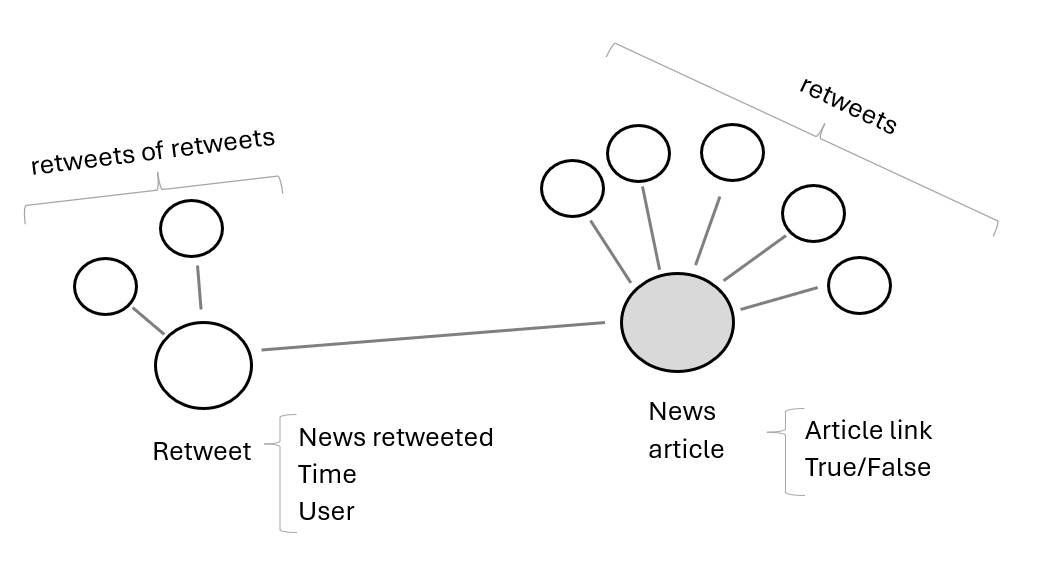
\includegraphics[width=0.48\textwidth]{struct}
	\end{center}
\end{wrapfigure}
\begin{itemize}
	\setlength\itemsep{-0.3em}
	\item \textbf{Graph Type}: Tree-structured graphs
	\item \textbf{Root Node}: News item (labeled true/false)
	\item \textbf{Other Nodes}: Twitter users who retweeted the news
	\item \textbf{Edges}:
	\begin{itemize}
		\setlength\itemsep{-0.3em}
		\item News item $\leftrightarrow$ User: Direct retweet
		\item User $\leftrightarrow$ User: Retweet through an intermediary
	\end{itemize}
	\item \textbf{Additional Information}: Retweet timestamps
\end{itemize}

The goal is to extract features from the network and use that data to train a machine learning model to predict the truthfulness of news.
The algorithms that we are going to use are important for:
\begin{itemize}
	\setlength\itemsep{-0.3em}
	\item \textbf{Average depth of trees}: Is the depth of the trees greater for fake news?
	\item \textbf{Average retweet breadth}: Do fake news tend to spread more quickly having a greater breadth at the first level?
	\item \textbf{Average time between retweets}: Do fake news spread faster?
	\item \textbf{Peak diffusion time}: Do fake news have an explosive peak?
	\item \textbf{Users reliability score}: various features based on the ranking of users who shared the news
	\item \textbf{Centrality and Pagerank}: What nodes are more common to find in paths between other 2 nodes?
\end{itemize}

\section*{Intended Experiments}

\subsection*{User reliability ranking}
\begin{wrapfigure}{r}{0.5\textwidth}
	\begin{center}
	  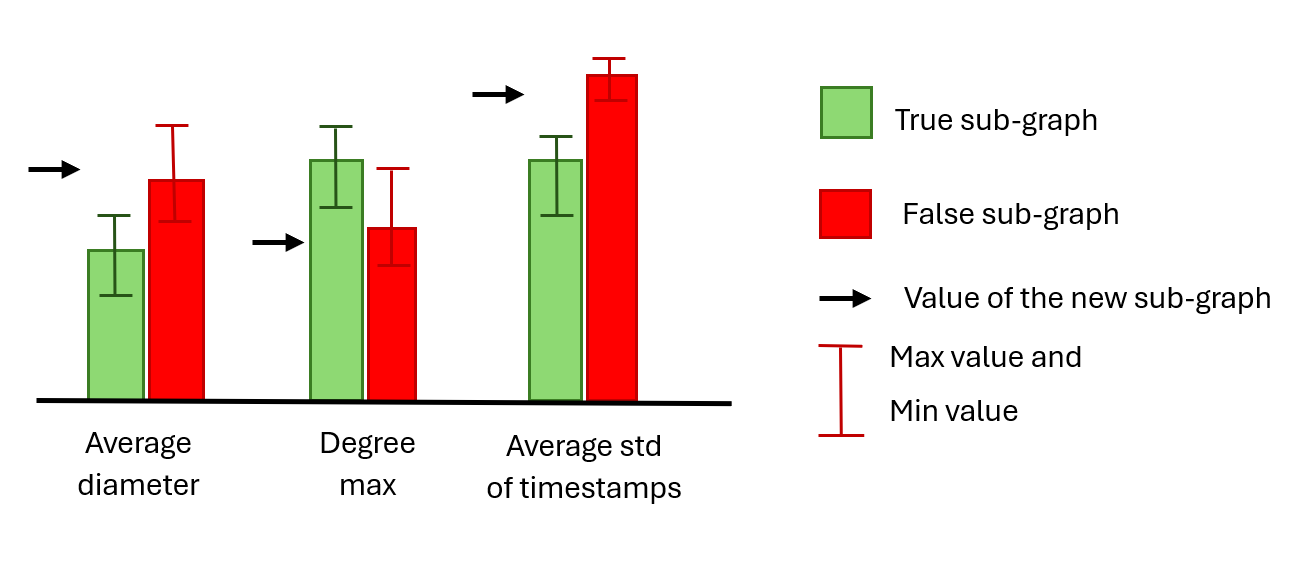
\includegraphics[width=0.48\textwidth]{results}
	\end{center}
\end{wrapfigure}
One of the goal is to visualize wether new data involving a news fits better into the "Real news" or "Fake news" category. This can be achieve displaying a bar graph representing the features studied previously.\\
The final step is to create a ranking of users based on their reliability and to generate features for the data using this ranking. More details about it will be given in the following pages.

\subsection*{Machine learning models}

The models we want to try are the following:
\begin{itemize}
	\setlength\itemsep{-0.3em}
	\item \textbf{Support Vector Machine}
	\item \textbf{Feed Forward Neural Network}
	\item \textbf{Random Forest}
\end{itemize}

We will make comparisons to better understand which model fits this problem best, based on which one achieves better accuracy and also the time it will take to train it.
\\\textbf{Libraries}: Networkx\cite{networkx} (for Graph analysis), Scikit-Learn\cite{scikit} (for SVM and RF models), Tensorflow\cite{tensor} (for FFNN model)
\\\textbf{Evaluation metrics of the model}: Accuracy, Precision, Recall and F1-Score
\\\textbf{Machine for experiments}: 
\begin{itemize}
	\setlength\itemsep{-0.3em}
	\item AMD Ryzen 5 3500U (8-cores), 8GB DDR4, Windows 11 or Ubunutu 20.04
	\item AMD Ryzen 5 4500 (8-cores), Radeon RX 6600, 16GB DDR4, Windows 11 or Ubuntu 20.04
\end{itemize}

\section*{Development}

\subsection*{Extracting informations from the dataset}

The first part of the project involves extracting the data from the datatset. As shown previously the dataset is composed of many connected components, each representing a news (related to gossip or politics). It has been decided, during the development, to consider only few features that could be relevant to the objective of the project.
Those features are:\\\\
\textbf{Diameter}: provides insight into the maximum extent of information spread. The bigger the diameter, the deeper (given that the structure of the graph is a tree) the news is spreaded among the users.\\
\textbf{Maximum degree}: identifies the node with the highest number of connections. In the case of fake news, such nodes could be targeted for spreading misinformation widely.\\
\textbf{Degree centrality}: the number of direct connections a node has. Nodes with high degree centrality are crucial in the immediate dissemination of news.\\
\textbf{Closeness centrality}: how quickly information can spread from a given node to all other nodes in the network. High closeness centrality suggests that a node is well-positioned to efficiently spread news.\\
\textbf{PageRank}: rank of nodes in a graph based on their importance. High PageRank nodes are influential and could be key disseminators of real or fake news.\\
\textbf{Average Standard Deviation of Retweet Timestamps}: consistency or burstiness of retweet activity over time. A small average standard deviation means that the news could be spreaded in a small amount of time since it has been tweeted for the first time.\\

Using networkx\cite{networkx} as the library for analyzing the graphs, extracting these information was actually easy. With all the features we then exported them into ".csv" files and ultimately we calculated all the average values separately for news labeled real and fake that are going to be used later in a system of prediction based on score.

\begin{lstlisting}[language=Python]
    import networkx as nx

    #calculating std of the timestamps
    std = np.std(np.array(timestamps))
    #calculating the diameter
    d = nx.diameter(s.graph)
    #calculating the max degree
    _, neighbors = max(s.graph.degree, key=lambda x: x[1])
    #calculating degree centrality
    dc = np.mean(list(nx.degree_centrality(s.graph).values()))
    #calculating closeness centrality
    cc = np.mean(list(nx.closeness_centrality(s.graph).values()))
    #calculating pagerank
    pr = np.mean(list(nx.pagerank(s.graph).values()))
\end{lstlisting}


\subsection*{\\Prediction system}
Once the features are extracted we have created a system based on score that is capable of predicting in a probabilistic way if a news is real or fake. This system gets some graphs data as input
and determines how much it deviates from the averages calculated with previous algorithms giving a final score from 0 to 12 (12 being the highest confidence).

\begin{lstlisting}[language=Python]
	def confidence_scoring(value, avg_r, avg_f):
        # Compute the difference
        diff_r = abs(avg_r - value)    #avg of real sub-graph - new value
        diff_f = abs(avg_f - value)    #avg of fake sub-graph - new value
        inside = (value<avg_r and value>avg_f) or (value<avg_f and value>avg_r) #The value is between the 2 avg
        #Closest one
        closer = 0              # 0 = Equal
        if diff_r < diff_f:
            closer = 1          # 1 = Real
        elif diff_r > diff_f:
            closer = 2          # 2 = Fake
        #Confidence score
        score = 0                                       #No guess
        if closer == 1:                                 #Real
            if 2*diff_r < diff_f or not inside:
                score = 2                               #Strong guess
            else:
                score = 1                               #Weak guess
        elif closer == 2:                               #Fake
            if 2*diff_f < diff_r or not inside:
                score = -2                              #Strong guess
            else:
                score = -1                              #Weak guess
        return score
\end{lstlisting}

\begin{center}
	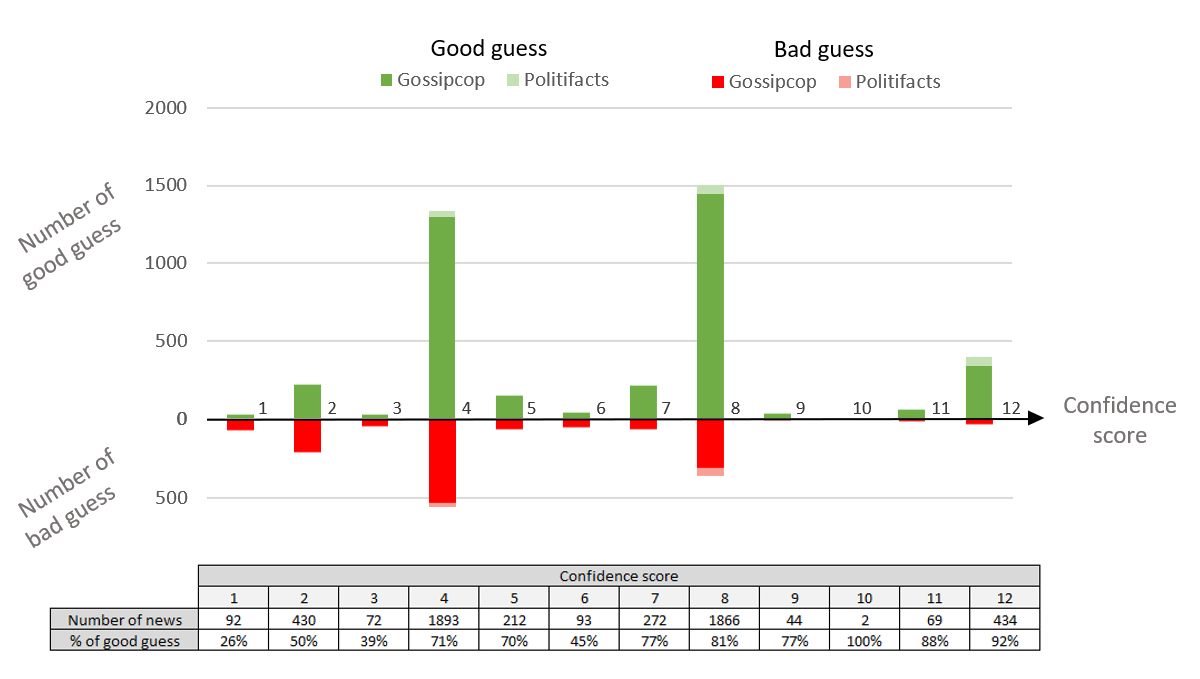
\includegraphics[width=0.8\textwidth]{graph}
\end{center}

The image above is just an example on how it can display the prediction and its accuracy. It represent
a confidence score on how sure we are about a news label. From what we can see, there is a correlation between the data extracted from
the graphs and their actual label. This is what we expected from the beginning so this will be important to develop a machine learning model which is able to predict the truthfulness of a news with a sufficiently high accuracy.

\subsection*{\\ \\User reliability ranking}
To enhance the prediction accuracy for our news dataset, we extended our feature set by incorporating user-related information in addition to the tree structure representing the news. Specifically, we developed a \textit{User Reliability Ranking} system, which captures key characteristics of users who shared the news.

\subsection*{Methodology}

The dataset was split into two parts: \textbf{Training set (80\%)} used to compute user-related features. \textbf{Test set (20\%)} used to measure the performance of the model using information about users taken from the training set.

\subsection*{Feature Extraction for Individual Users}
For each user in the training set, we calculated the following features, considering that a user who shares multiple news items will appear in several news trees:
\begin{enumerate}
    \item \textbf{Number of fake news retweets}
    \item \textbf{Number of true news retweets}
    \item \textbf{Total number of retweets}
    \item \textbf{Average PageRank Centrality} across all trees where the user appears.
    \item \textbf{Average Degree Centrality} across all trees where the user appears.
    \item \textbf{Average Closeness Centrality} across all trees where the user appears.
    \item \textbf{User Score}, calculated as follows:
    
\end{enumerate}

\begin{center}
	UserScore = US \\
	Normalized number of false retweets = FR \\
	Normalized true to false ratio = TFR \\
	Normalized pagerank of node = NP \\
	Normalized degree centrality of node = DC \\
	Normalized closeness centrality of node = CC \\
\end{center}

\begin{equation}
	US = 0.4 \times FR + 0.3 \times TFR + 0.1 \times NP + 0.1 \times DC + 0.1 \times CC
\end{equation}

\subsection*{Feature Aggregation for News Trees}
For each news tree in the dataset, we derived features based on the users who shared that news, utilizing the \textit{User Reliability Ranking} described above. These features include:
\begin{itemize}
    \item \textbf{Average User Score} of all users who shared the news.
    \item \textbf{Percentage of reliable users} (users exceeding an experimentally determined User Score threshold).
    \item \textbf{Minimum User Score} among users who shared the news.
    \item \textbf{Maximum User Score} among users who shared the news.
    \item \textbf{Average PageRank Centrality} of users who shared the news.
    \item \textbf{Average Degree Centrality} of users who shared the news.
    \item \textbf{Average Closeness Centrality} of users who shared the news.
\end{itemize}

\subsection*{Model Training and Testing}
These user-related features were combined with the existing tree structure features to train the model. During the training phase, user-related features were computed exclusively using the training set.

In the testing phase, we computed the user-related features for the test set using only the user information derived from the training set.

\subsection*{Results}
Incorporating the user-related features significantly improved the model's accuracy compared to the baseline model that used only tree structure features. Below are the results of the models trained with the "gossipcop" dataset.

\begin{table}[ht]
\centering
\begin{tabular}{|c|c|c|c|c|}
\hline
Class & Precision & Recall & F1-Score & Support \\
\hline
0.0    & 0.88      & 0.85   & 0.86     & 580     \\
1.0    & 0.83      & 0.87   & 0.85     & 513     \\
\hline
\textbf{Accuracy}   & \multicolumn{4}{c|}{0.86 (1093)} \\
\hline
Macro avg           & 0.86      & 0.86   & 0.86     & 1093    \\
Weighted avg        & 0.86      & 0.86   & 0.86     & 1093    \\
\hline
\end{tabular}
\caption{Random Forest without using User Reliability Ranking}
\end{table}

\begin{table}[ht]
\centering
\begin{tabular}{|c|c|c|c|c|}
\hline
Class & Precision & Recall & F1-Score & Support \\
\hline
0.0    & 0.85      & 0.86   & 0.85     & 561     \\
1.0    & 0.85      & 0.84   & 0.84     & 532     \\
\hline
\textbf{Accuracy}   & \multicolumn{4}{c|}{0.85 (1093)} \\
\hline
Macro avg           & 0.85      & 0.85   & 0.85     & 1093    \\
Weighted avg        & 0.85      & 0.85   & 0.85     & 1093    \\
\hline
\end{tabular}
\caption{Feed Forward Neural Network without using User Reliability Ranking}
\end{table}


\begin{table}[ht]
\centering
\begin{tabular}{|c|c|c|c|c|}
\hline
Class & Precision & Recall & F1-Score & Support \\
\hline
0.0    & 0.84      & 0.80   & 0.82     & 547     \\
1.0    & 0.81      & 0.85   & 0.83     & 547     \\
\hline
\textbf{Accuracy}   & \multicolumn{4}{c|}{0.82 (1094)} \\
\hline
Macro avg           & 0.83      & 0.82   & 0.82     & 1094    \\
Weighted avg        & 0.83      & 0.82   & 0.82     & 1094    \\
\hline
\end{tabular}
\caption{SVM Polynomial Kernel without using User Reliability Ranking}
\end{table}

\newpage

The Support Vector Machine results were promising even though the model is very simple, requires few resources and the training is not time consuming. We then tried to concatenate the User ranking data to the features of the news graph and feed them into another SVM model with the same parameters as the one used in figure (a). The results were impressive:

\begin{table}[ht]
\centering
\begin{tabular}{|c|c|c|c|c|}
\hline
Class & Precision & Recall & F1-Score & Support \\
\hline
0.0    & 0.96      & 0.88   & 0.92     & 547     \\
1.0    & 0.89      & 0.96   & 0.92     & 547     \\
\hline
\textbf{Accuracy}   & \multicolumn{4}{c|}{0.92 (1094)} \\
\hline
Macro avg           & 0.92      & 0.92   & 0.92     & 1094    \\
Weighted avg        & 0.92      & 0.92   & 0.92     & 1094    \\
\hline
\end{tabular}
\caption{SVM Polynomial Kernel (C=10, degree=3), with data from User Reliability Ranking}
\end{table}
\subsection*{Challanges encountered}
The most challenging part was extracting the data, as much of the information in the dataset—like user IDs and news labels—is spread across multiple files. Ensuring consistency while retrieving this data took significant effort. Initially, a mistake was made during the model training process: the User Ranking was calculated using the entire dataset, including the portion later designated as the test set. As a result, the test set already contained pre-extracted user information derived during the User Ranking calculation. This led to artificially inflated performance results, an indication of overfitting. To address this, we corrected the process by calculating the User Ranking solely on the training set while leaving the test set untouched. Due to the added complexity, we skipped k-fold cross-validation for models using the User Ranking, unlike those trained without it. Implementing this would have required recalculating the ranking dynamically for each fold, which was infeasible given time constraints. Instead, we reused hyperparameters from the models trained without the User Ranking. Future development could focus on integrating this functionality into the code.
\subsection*{Conclusions}
This study successfully demonstrated that fake news on Twitter can be identified using graph-based features without relying on user metadata. Key features such as tree depth, retweet breadth, and centrality metrics were extracted and used to train machine learning models, achieving high accuracy. The integration of a User Reliability Ranking further improved model performance, boosting precision, recall, and overall predictive accuracy to 92\% using an SVM with user data.
\\These results show the effectiveness of using retweet graph structures for misinformation detection.







\newpage

\begin{thebibliography}{9}
	\bibitem{rec_studies} Yi Han, Shanika Karunasekeran, Christopher Leckie\\"Graph Neural Networks with Continual Learning for Fake News Detection from Social Media",\\ \url{https://arxiv.org/pdf/2007.03316}, 2020.
	\bibitem{dataset} Dataset: \url{https://github.com/safe-graph/GNN-FakeNews/tree/main},\\\url{https://drive.google.com/drive/folders/1OslTX91kLEYIi2WBnwuFtXsVz5SS_XeR?usp=sharing}
	\bibitem{data_paper} Kai Shu, Deepak Mahudeswaran, Suhang Wang, Dongwon Lee and Huan Liu\\"FakeNewsNet: A Data Repository with News Content, Social Context and Spatiotemporal Information for Studying Fake News on Social Media",\\ \url{https://arxiv.org/pdf/1809.01286}, 2019
	\bibitem{networkx} NetworkX library: \url{https://networkx.org/documentation/stable/}
	\bibitem{scikit} Scikit-learn library: \url{https://scikit-learn.org/stable/api/index.html}
	\bibitem{tensor} Tensorflow library: \url{https://www.tensorflow.org/api_docs/python/tf}
\end{thebibliography}

\newpage

\section*{Contribution}
Contributors:
\begin{itemize}
	\setlength\itemsep{-0.3em}
	\item Baggio Davide ($\frac{1}{3}$ of the work): Finding a well documented dataset, reading the related papers and understanding it. Writing the first part of the proposal and preprocessing the dataset ready for analysis into a python script.
	\item Martinez Zoren ($\frac{1}{3}$ of the work): Finding a well documented dataset,  reading the related papers and understanding it. Writing the third part of the proposal and planning on the machine learning models to use in order to achieve the goal of the project.
	\item Brocheton Damien ($\frac{1}{3}$ of the work): Finding a well documented dataset,  reading the related papers and understanding it. Writing the second part of the proposal and starting to write the postprocessing of the data into a python script that compare new data with the studied one using a probabilistic algorithm.
\end{itemize}

\end{document}
